\documentclass[compress]{beamer}
\usecolortheme{default}

\usepackage{lmodern, epstopdf, multirow, array, setspace, bbm, tcolorbox, pbox, bm, mathtools, tikz}
\usepackage[T1]{fontenc}

\setbeamertemplate{frametitle}[default][center]
\setbeamertemplate{footline}{\hfill \insertframenumber/\inserttotalframenumber\hspace*{5pt}\vspace{5pt}}
\setbeamertemplate{navigation symbols}{}

\newlength{\wideitemsep}
\setlength{\wideitemsep}{\itemsep}
\addtolength{\wideitemsep}{4pt}
\let\olditem\item
\renewcommand{\item}{\setlength{\itemsep}{\wideitemsep}\olditem}
\setlength{\leftmargini}{12pt}
\setlength{\leftmarginii}{14pt}
\setbeamertemplate{itemize/enumerate subbody begin}{\vspace{6pt}}
\setbeamertemplate{itemize item}[circle]
\setbeamertemplate{enumerate item}[circle]
\setbeamertemplate{enumerate subitem}[default]

\setbeamercolor{alerted text}{fg=blue}
\setbeamersize{text margin left=1.5em,text margin right=1.5em}

\tcbset{
    colback=white,
    colframe=black,
    coltext=black,
    coltitle=blue,
    colbacktitle=white,
    boxrule=1pt,
    titlerule=0pt,
    toptitle=4pt,
    top=2pt
}

\newenvironment{changemargin}[2]{% 
  \begin{list}{}{% 
    \setlength{\topsep}{0pt}% 
    \setlength{\leftmargin}{#1}% 
    \setlength{\rightmargin}{#2}% 
    \setlength{\listparindent}{\parindent}% 
    \setlength{\itemindent}{\parindent}% 
    \setlength{\parsep}{\parskip}% 
  }% 
  \item[]}{\end{list}}
  
\newenvironment{defn}{%
  \begin{tcolorbox}[title={Definition}]%
  }{\end{tcolorbox}}
  
\newenvironment{prop}[1]{%
  \begin{tcolorbox}[title={Proposition #1}]%
  }{\end{tcolorbox}}
  
\newcommand{\cit}[1]{{\footnotesize \textcolor[rgb]{0.5,0,0}{#1}}}

% Font size for code listings (verbatim blocks); reset with \normalsize
\newcommand{\codesize}{\fontsize{7}{8.5}\selectfont}

\newcommand{\slidesetup}[1]{%
  \title{#1}%
  \subtitle{\texorpdfstring{\vspace{0.3\baselineskip}}{} {\small This version: \today}}%
  \author[Mikkel Plagborg-Moller]{ECMA 31150, Spring 2026 \texorpdfstring{\\[0.5ex]}{} University of Chicago \texorpdfstring{\\[0.5ex]}{} Department of Economics \texorpdfstring{\\[4ex]}{} Mikkel Plagborg-Moller}%
  \date{}%
}

% \circleoverlay[options]{text}
% Draws a red circle with a text box nearby on a tikz overlay.
% Options (with defaults):
%   cx=0cm, cy=0cm      - circle center (shift from page center)
%   r=1cm               - circle radius
%   tx=0cm, ty=0cm      - text box offset from circle center
%   text anchor=east    - anchor of text node (east = text left, west = text right)
%   font=\normalsize    - font size for text
\pgfkeys{
  /circleoverlay/.cd,
  cx/.store in=\cocx, cx=0cm,
  cy/.store in=\cocy, cy=0cm,
  r/.store in=\cor, r=1cm,
  tx/.store in=\cotx, tx=0cm,
  ty/.store in=\coty, ty=0cm,
  text anchor/.store in=\cotextanchor, text anchor=east,
  font/.store in=\cofont, font=\normalsize,
}
\newcommand{\circleoverlay}[2][]{%
  \pgfkeys{/circleoverlay/.cd, cx=0cm, cy=0cm, r=1cm, tx=0cm, ty=0cm, text anchor=east, font=\normalsize, #1}%
  \pgfmathsetlengthmacro{\circlediameter}{2*\cor}%
  \node[draw=red, line width=2pt, circle, minimum size=\circlediameter, inner sep=0pt]
    (tmpcirc) at ([xshift=\cocx,yshift=\cocy]current page.center) {};%
  \node[anchor=\cotextanchor, fill=white, draw=red, text=red, inner sep=4pt, align=left, font=\cofont]
    at ([xshift=\cotx,yshift=\coty]tmpcirc.center) {#2};%
}

\DeclareMathOperator*{\argmax}{argmax}
\DeclareMathOperator*{\argmin}{argmin}
\DeclareMathOperator{\diag}{diag}
\DeclareMathOperator{\var}{Var}
\DeclareMathOperator{\cov}{Cov}
\DeclareMathOperator{\corr}{Corr}
\DeclareMathOperator{\lrv}{LRV}

\usetikzlibrary{positioning, fit, arrows.meta, shapes.geometric}

\slidesetup{Dynamic causal effects III}

\begin{document}
\frame{
\maketitle
}

\frame{
\frametitle{Plan for this slide deck}
\begin{enumerate}
\item Using VARs for causal inference
\item Application: monetary policy shocks
\item VAR vs.\ LP estimators
\item Other identification approaches
\end{enumerate}
}

\frame{
\frametitle{Structural VAR}
\begin{itemize}
\item Assume we have an $n \times 1$ data vector $\bm{y}_t$ whose dynamics are well described by a VAR (here 1 lag for simplicity):
\begin{equation} \label{eqn:var}
\bm{y}_t = \bm{c} + \bm{A}\bm{y}_{t-1} + \bm{u}_t,\quad \bm{u}_t \sim \mathit{WN}(\bm{\Sigma}). \tag{$\dagger$}
\end{equation}
\item The elements of $\bm{u}_t$ are forecast errors, \emph{not} structural shocks.
\item But let's now assume that the forecast errors are linear combinations of some underlying, unobserved structural shocks:
\begin{equation} \label{eqn:shocks}
\bm{u}_t = \bm{H}\bm{\varepsilon}_t,\quad \bm{\varepsilon}_t \sim \mathit{WN}(\bm{I}). \tag{$\ddagger$}
\end{equation}
\item It's conventional to assume that $\bm{\varepsilon}_t$ is also $n \times 1$. Then $\bm{H}$ is $n \times n$, and $\bm{I}$ is the $n \times n$ identity matrix.
\begin{itemize}
\item Note: now we normalize $\var(\varepsilon_{jt})=1$ for all $j=1,\dots,n$.
\end{itemize}
\item The model (\ref{eqn:var})--(\ref{eqn:shocks}) is called a \textbf{structural VAR} (SVAR).
\end{itemize}
}

\frame{
\frametitle{IRFs}
\[\bm{y}_t = \bm{c} + \bm{A}\bm{y}_{t-1} + \bm{H}\bm{\varepsilon}_t,\quad \bm{\varepsilon}_t \sim \mathit{WN}(\bm{I})\]
\begin{itemize}
\item \alert{Exercise:} the (stationary) SVAR model implies the SVMA representation
\[\bm{y}_t = \bm{\mu} + \sum_{\ell=0}^\infty \bm{\Theta}_\ell \bm{\varepsilon}_{t-\ell}, \quad \text{where} \quad \bm{\mu} \equiv (\bm{I}-\bm{A})^{-1}\bm{c},\quad \bm{\Theta}_\ell \equiv \bm{A}^\ell \bm{H}.\]
(Each of the variables $y_{1t},\dots,y_{nt}$ satisfies an SVMA model.)
\item Impulse response at horizon $h$ of the $i$-th variable $\lbrace y_{it} \rbrace$ wrt.\ the $j$-th shock $\lbrace \varepsilon_{jt} \rbrace$: $(i,j)$ element of $\boxed{\bm{\Theta}_h = \bm{A}^h\bm{H}}$.
\item In particular, the \emph{impact} impulse responses ($h=0$) are just $\bm{\Theta}_0=\bm{H}$.
\end{itemize}
}

\frame{
\frametitle{FEVD}
\begin{itemize}
\item $h$-step-ahead forecast error:
\[\bm{y}_{t+h} - \bm{y}_{t+h|t} = \sum_{\ell=0}^{h-1} \bm{A}^\ell \bm{u}_{t+h-\ell} = \sum_{\ell=0}^{h-1} \bm{A}^\ell \bm{H}\bm{\varepsilon}_{t+h-\ell}.\]
\item Let $\bm{e}_i$ be the $i$-th column of the $n \times n$ identity matrix $\bm{I}$.
\item Fraction of forecast error variance of $y_{i,t+h}$ contributed by the sequence $\varepsilon_{j,t+1},\dots,\varepsilon_{j,t+h}$ of the $j$-th shock:
\[\mathit{FEVD}_{h,ij} \equiv \frac{\var\left(\bm{e}_i'\sum_{\ell=0}^{h-1} \bm{A}^\ell \bm{H}\bm{e}_j\varepsilon_{j,t+h-\ell}\right)}{\var\left(\bm{e}_i'\sum_{\ell=0}^{h-1} \bm{A}^\ell \bm{H}\bm{\varepsilon}_{t+h-\ell}\right)} = \boxed{\frac{\sum_{\ell=0}^{h-1} (\bm{e}_i'\bm{A}^\ell \bm{H}\bm{e}_j)^2}{\sum_{\ell=0}^{h-1} \bm{e}_i'\bm{A}^\ell \bm{\Sigma}(\bm{A}^\ell)'\bm{e}_i}},\]
where $\bm{\Sigma} \equiv \var(\bm{u}_t) = \bm{H}\bm{H}'$.
\begin{itemize}
\item \alert{Exercise:} verify the final expression above for the FEVD.
\end{itemize}
\end{itemize}
}

\frame{
\frametitle{SVAR identification}
\[\bm{y}_t = \bm{c} + \bm{A}\bm{y}_{t-1} + \bm{u}_t,\quad \bm{u}_t = \bm{H}\bm{\varepsilon}_t,\quad \bm{\varepsilon}_t \sim \mathit{WN}(\bm{I})\]
\vspace{-0.5\baselineskip}
\begin{itemize}
\item Since $\lbrace \bm{u}_t \rbrace$ is white noise, we learned previously that we can consistently estimate $\bm{c}$ and $\bm{A}$ with the OLS estimators $\hat{\bm{c}}$ and $\hat{\bm{A}}$.
\item The final ingredient for estimating IRFs and FEVDs is $\bm{H}$. How to estimate it?
\item As on the previous slide,
\begin{equation} \label{eqn:svar_identif}
\bm{\Sigma} \equiv \var(\bm{u}_t) = \bm{H}\bm{H}'. \tag{$\ast$}
\end{equation}
\item Recall that the sample var-cov matrix of the residuals, $\hat{\bm{\Sigma}}$, is a consistent estimator of $\bm{\Sigma}$.
\item Given the estimate of $\bm{\Sigma}$, can we use equation (\ref{eqn:svar_identif}) to solve for $\bm{H}$?
\end{itemize}
}

\frame{
\frametitle{SVAR identification (cont.)}
\[\bm{\Sigma} = \bm{H}\bm{H}'\]
\vspace{-0.5\baselineskip}
\begin{itemize}
\item This matrix equation has $n^2$ unknowns: the elements of $\bm{H}$.
\item But there are only $\frac{n(n+1)}{2}$ equations, which is less than $n^2$ (if $n>1$).
\item Why are there not $n^2$ equations? Because $\bm{\Sigma}$ is necessarily symmetric, so the equations above the diagonal are redundant given the equations below the diagonal.
\item Conclusion: we don't have enough equations to pin down $\bm{H}$. The IRFs are \textbf{not identified}.
\end{itemize}
}

\frame{
\frametitle{Identification from timing restrictions}
\begin{itemize}
\item We need to make more assumptions if we want to identify $\bm{H}$.
\item As in the first slide deck on local projections, we may be willing to assume some \textbf{short-run timing restrictions}: restrict which variables $y_{it}$ can respond to which shocks $\varepsilon_{jt}$ on impact.
\item Consider ``recursive'' timing assumptions:
\[y_{it} \quad \text{does not respond to} \quad \varepsilon_{i+1,t},\varepsilon_{i+2,t},\dots,\varepsilon_{n,t} \quad \text{on impact},\]
for $i=1,2,\dots,n-1$.
\item The last variable $y_{nt}$ can respond to all shocks on impact.
\end{itemize}
}

\frame{
\begin{figure}
Example with $n=3$:
\bigskip

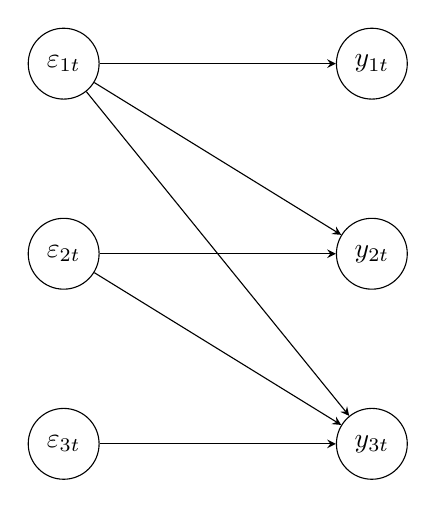
\begin{tikzpicture}[
    node distance=1.5cm and 3cm,
    shock/.style={circle, draw, minimum size=0.9cm, inner sep=1pt},
    var/.style={circle, draw, minimum size=0.9cm, inner sep=1pt},
    >=stealth
]
% Shocks (left column)
\node[shock] (e1) {$\varepsilon_{1t}$};
\node[shock, below=of e1] (e2) {$\varepsilon_{2t}$};
\node[shock, below=of e2] (e3) {$\varepsilon_{3t}$};

% Variables (right column)
\node[var, right=of e1] (y1) {$y_{1t}$};
\node[var, right=of e2] (y2) {$y_{2t}$};
\node[var, right=of e3] (y3) {$y_{3t}$};

% Recursive structure: epsilon_i affects y_j for j >= i
 \foreach \j/\ymin in {1/1, 2/2, 3/3}
   \foreach \i in {\ymin,...,3}
     \draw[->] (e\j) -- (y\i);
\end{tikzpicture}
\end{figure}
}

\frame{
\frametitle{Identification from timing restrictions (cont.)}
\begin{itemize}
\item Mathematically, these timing assumptions mean that the impact impulse response matrix $\bm{\Theta}_0 = \bm{H}$ is \textbf{lower triangular}:
\[\bm{H} = \begin{pmatrix}
H_{11} & 0 & \cdots & \cdots & 0 \\
H_{21} & H_{22} & 0 & \cdots & 0 \\
\vdots & & \ddots & \ddots & \vdots \\
H_{n-1,1} & H_{n-1,2} & \cdots & H_{n-1,n-1} & 0 \\
H_{n1} & H_{n2} & \cdots & H_{n,n-1} & H_{nn}
\end{pmatrix}.\]
\item Also assume the diagonal is positive: $H_{ii}>0$ for $i=1,\dots,n$.
\begin{itemize}
\item This just normalizes the sign of the shock so that $y_{it}$ responds positively to $\varepsilon_{it}$ on impact.
\end{itemize}
\end{itemize}
}

\frame{
\frametitle{Identification from timing restrictions (cont.)}
\begin{itemize}
\item \alert{Result} (from linear algebra): the matrix equation
\[\bm{\Sigma} = \bm{H}\bm{H}'\]
has a \emph{unique} lower triangular solution $\bm{H}$ with positive diagonal.
\item The solution is called the \textbf{Cholesky factor} of $\bm{\Sigma}$, and efficient numerical algorithms exist.
\begin{itemize}
\item Python: \texttt{numpy.linalg.cholesky}
\end{itemize}
\item So we can estimate $\hat{\bm{H}} \equiv \text{Cholesky}(\hat{\bm{\Sigma}})$.
\item Identification from short-run timing restrictions is also called ``Cholesky'' or ``recursive'' identification.
\end{itemize}
}

\frame{
\frametitle{Summary: SVAR estimation of IRF and FEVD}
\begin{enumerate}
\item Estimate $\hat{\bm{A}}$ and $\hat{\bm{\Sigma}}$ by OLS (same as earlier slides on forecasting).
\item Compute $\hat{\bm{H}} \equiv \text{Cholesky}(\hat{\bm{\Sigma}})$.
\item Impulse response estimator:
\[\hat{\bm{\Theta}}_h \equiv \hat{\bm{A}}^h\hat{\bm{H}}.\]
\vspace{-1.5\baselineskip}
\begin{itemize}
\item If VAR is in $(np) \times (np)$ companion form, only apply Cholesky to $n \times n$ matrix $\hat{\bm{\Sigma}}$ and then pad $\hat{\bm{H}}$ below with zeros.
\end{itemize}
\item FEVD estimator:
\[\widehat{\mathit{FEVD}}_{h,ij} \equiv \frac{\sum_{\ell=0}^{h-1} (\bm{e}_i'\hat{\bm{A}}^\ell \hat{\bm{H}}\bm{e}_j)^2}{\sum_{\ell=0}^{h-1} \bm{e}_i'\hat{\bm{A}}^\ell \hat{\bm{\Sigma}}(\hat{\bm{A}}^\ell)'\bm{e}_i}.\]
\end{enumerate}
\begin{itemize}
\item These estimators are just functions of $(\hat{\bm{A}},\hat{\bm{\Sigma}})$. So we can compute bootstrap confidence intervals as in our earlier slide deck on VARs.
\end{itemize}
}

\frame{
\frametitle{Single-shock identification}
\begin{itemize}
\item For the Cholesky decomposition, the ordering of the variables in $\bm{y}_t$ matters. The ordering encodes our assumptions about which shocks can affect each variable.
\item If you want to identify the IRFs wrt.\ all the $n$ shocks in $\bm{\varepsilon}_t$, you have to justify your specific variable ordering by defending many timing restrictions ($\frac{n(n-1)}{2}$ of them).
\item But suppose you only care about a single shock, say, the $j$-th one.
\item Then it turns out that for the Cholesky decomposition, the ordering \emph{among} the earlier variables $y_{1t},\dots,y_{j-1,t}$ does not matter, and neither does the ordering \emph{among} the later variables $y_{j+1,t},\dots,y_{nt}$.
\end{itemize}
}

\frame{
\frametitle{Single-shock identification (cont.)}
\begin{itemize}
\item As a consequence, when estimating the IRFs and FEVDs for a single shock $j$, we ``only'' need to assume:
\begin{enumerate}
\item The first $j-1$ variables $y_{1t},\dots,y_{j-1,t}$ do not respond to the last $n-j+1$ shocks $\varepsilon_{jt},\dots,\varepsilon_{nt}$ on impact.
\item The $j$-th variable $y_{jt}$ does not respond to the last $n-j$ shocks $\varepsilon_{j+1,t},\dots,\varepsilon_{nt}$ on impact.
\end{enumerate}
\item In practice, it is often difficult enough to defend these timing assumptions for single-shock identification.
\item Trying to identify all $n$ shocks via recursive timing restrictions is rarely credible, though many papers try\dots
\end{itemize}
}

\frame{
\begin{figure}
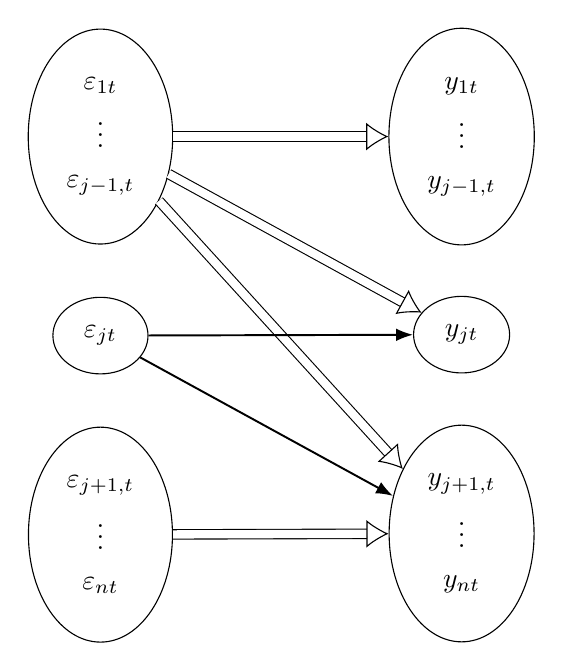
\begin{tikzpicture}[
    >=Latex,
    mynode/.style={inner sep=2pt},
    group/.style={draw, ellipse, inner sep=4pt},
    multiarrow/.style={
        -{Latex[open, length=8pt, width=10pt]},
        double, double distance=3pt,
        line width=0.4pt
    },
    singlearrow/.style={->, line width=0.7pt}
]

% Shock column (left)
\node[mynode] (eA1) {$\varepsilon_{1t}$};
\node[mynode, below=0cm of eA1] (eA2) {$\vdots$};
\node[mynode, below=0.2cm of eA2] (eA3) {$\varepsilon_{j-1,t}$};

\node[mynode, below=1.5cm of eA3] (eB) {$\alert{\varepsilon_{jt}}$};

\node[mynode, below=1.5cm of eB] (eC1) {$\varepsilon_{j+1,t}$};
\node[mynode, below=0cm of eC1] (eC2) {$\vdots$};
\node[mynode, below=0.2cm of eC2] (eC3) {$\varepsilon_{nt}$};

\node[group, fit=(eA1) (eA3)] (gEa) {};
\node[group, fit=(eB)] (gEb) {};
\node[group, fit=(eC1) (eC3)] (gEc) {};

% Variable column (right)
\node[mynode, right=4cm of eA1] (yA1) {$y_{1t}$};
\node[mynode, below=0cm of yA1] (yA2) {$\vdots$};
\node[mynode, below=0.2cm of yA2] (yA3) {$y_{j-1,t}$};

\node[mynode, below=1.48cm of yA3] (yB) {$y_{jt}$};

\node[mynode, below=1.49cm of yB] (yC1) {$y_{j+1,t}$};
\node[mynode, below=0cm of yC1] (yC2) {$\vdots$};
\node[mynode, below=0.2cm of yC2] (yC3) {$y_{nt}$};

\node[group, fit=(yA1) (yA3)] (gYa) {};
\node[group, fit=(yB)] (gYb) {};
\node[group, fit=(yC1) (yC3)] (gYc) {};

% Arrows from gEa (multiple shocks): wide hollow
\draw[multiarrow] (gEa) -- (gYa);
\draw[multiarrow] (gEa) -- (gYb);
\draw[multiarrow] (gEa) -- (gYc);

% Arrows from gEb (single shock): thin
\draw[singlearrow] (gEb) -- (gYb);
\draw[singlearrow] (gEb) -- (gYc);

% Arrows from gEc (multiple shocks): wide hollow
\draw[multiarrow] (gEc) -- (gYc);
\end{tikzpicture}
\end{figure}
}

\frame{
\frametitle{Application: identification of monetary policy shocks}
\begin{itemize}
\item We follow a classic approach to identify the causal effects of monetary policy (MP) shocks: movements in the federal funds rate beyond the systematic policy rule.
\item Recursive SVAR identification with the following ordering ($n=6$):
\[\bm{y}_t = \begin{pmatrix}
\log(\text{INDPRO}_t) \\
\text{UNRATE}_t \\
\log(\text{CPI}_t) \\
\log(\text{PCOM}_t) \\
\alert{\text{FEDFUNDS}_t} \\
\text{NFCI}_t
\end{pmatrix}.\]
\item INDPRO: industrial production. UNRATE: unemployment rate. PCOM: commodity price index. NFCI: financial conditions index.
\end{itemize}
}

\frame{
\frametitle{Application: monetary policy shocks (cont.)}
\begin{itemize}
\item FEDFUNDS ordered 5th. MP shock $\equiv \varepsilon_{5t}$.
\item ``Slow-moving'' variables ordered \emph{before} FEDFUNDS: INDPRO, UNRATE, CPI, PCOM.
\item ``Fast-moving'' variable ordered \emph{after} FEDFUNDS: NFCI.
\item Timing assumptions for identifying MP shock (certainly debatable!):
\begin{enumerate}
\item Slow-moving variables do not respond on impact to the MP shock $\varepsilon_{5t}$ or to the financial shock $\varepsilon_{6t}$. Could be justified theoretically based on economic adjustment costs and nominal rigidities in prices.
\item FEDFUNDS (the MP instrument) does not react to the financial shock $\varepsilon_{6t}$ on impact. Could be justified by the Fed claiming that they ``see through'' short-term movements in financial markets.
\end{enumerate}
\end{itemize}
}

\begin{frame}[fragile]
\scriptsize
\begin{verbatim}
# Estimate VAR
order = ['l_INDPRO', 'UNRATE', 'l_CPIAUCSL', 'l_PCOM', 'FEDFUNDS', 'NFCI']
nlag = 12
model = sm.tsa.VAR(df[order])
res = model.fit(maxlags=nlag, ic=None) # fix lag length

# Cholesky-identified IRFs
max_horizon = 48
irf = res.irf(max_horizon)

# FEVD
fevd = res.fevd(max_horizon)
\end{verbatim}
\normalsize
\bigskip
\begin{itemize}
\item The structural impulse response at horizon $h$ of variable $i$ wrt.\ shock $j$ is stored in \texttt{irf.orth\_irfs[h,i-1,j-1]}.
\begin{itemize}
\item ``Orth'': orthogonalized. The structural shocks $\varepsilon_{jt}$, $j=1,\dots,n$, are orthogonal to each other (i.e., mutually uncorrelated).
\end{itemize}
\item The FEVD is stored in \texttt{fevd.decomp[i-1, h-1, j-1]}.
\end{itemize}
\end{frame}

\frame{
\begin{center}
\textbf{IRFs to 1-standard-deviation monetary policy shock}
\end{center}
\vspace{-0.5\baselineskip}
\begin{figure}
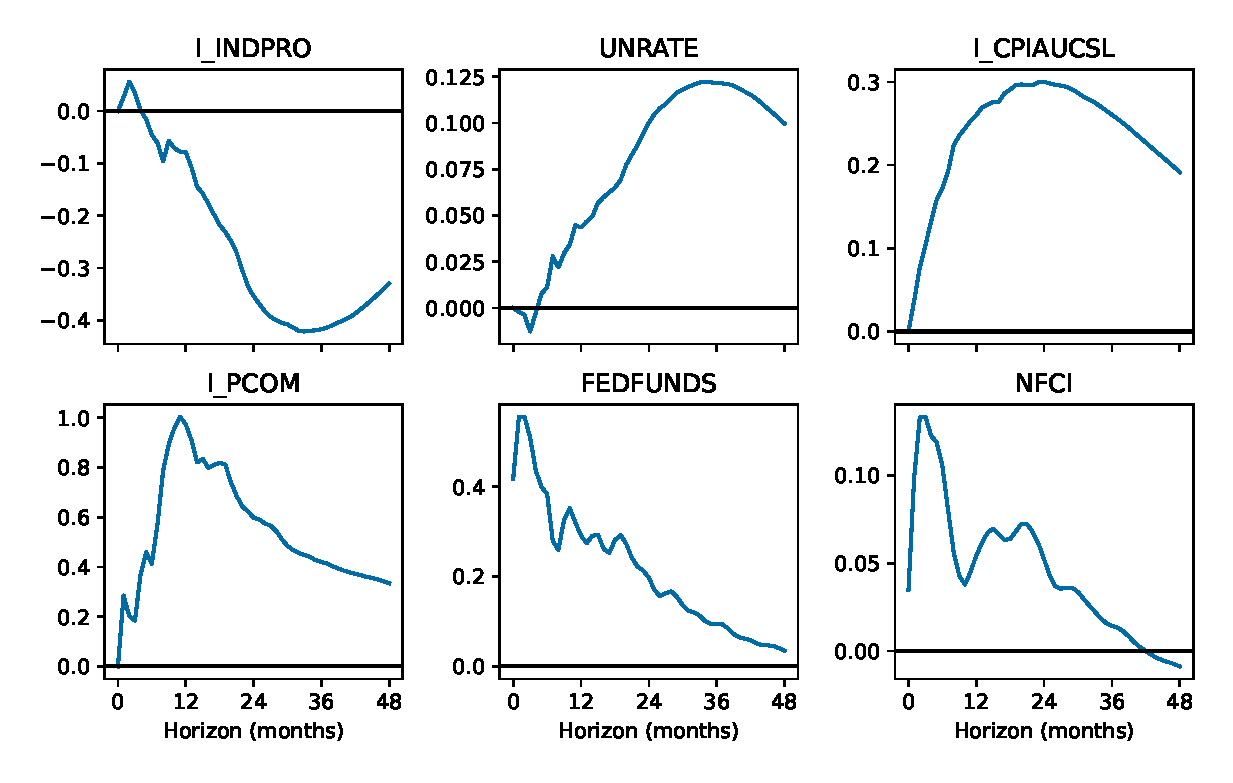
\includegraphics[width=\linewidth]{fig/mpshock_irf.eps}
\end{figure}
}

\frame{
\begin{center}
\textbf{FEVD share of monetary policy shock}
\end{center}
\vspace{-0.5\baselineskip}
\begin{figure}
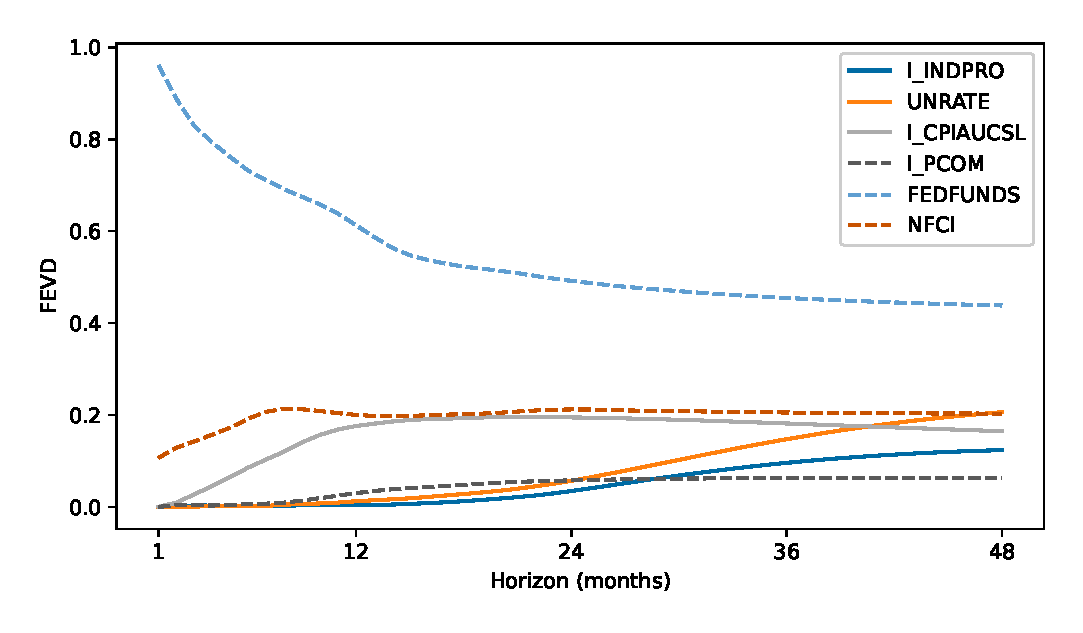
\includegraphics[width=\linewidth]{fig/mpshock_fevd.eps}
\end{figure}
}

\frame{
\frametitle{Trending variables}
\begin{itemize}
\item In the application my VAR included variables with clear time trends, like industrial production.
\item While our theory assumed stationary $\bm{y}_t$, it turns out that one can still compute IRFs and FEVDs using our previous formula even if $\bm{A}$ does not have all eigenvalues inside the unit circle.
\item In most cases, we can also use our normal VAR bootstrap even when the variables have stochastic trends.
\item We will discuss non-stationary models explicitly later in the course.
\end{itemize}
}

\frame{
\frametitle{Directly measured shock}
\begin{itemize}
\item Suppose we directly observe a shock $x_t=\varepsilon_{1t}$.
\item Then we can order it first in a recursive SVAR:
\[\bm{y}_t = (x_t,y_{2t},y_{3t},\dots,y_{nt})'.\]
\item Since there are no variables ordered before $x_t$, the timing assumption is just: $x_t$ does not respond to other shocks than $\varepsilon_{1t}$ on impact. This is automatically satisfied if we have correctly measured the shock!
\item So we can report Cholesky-orthogonalized IRFs and FEVDs wrt.\ the first shock in the SVAR.
\begin{itemize}
\item The ordering of the other variables does not matter.
\end{itemize}
\end{itemize}
}

\frame{
\frametitle{Proxies}
\begin{itemize}
\item Now suppose we want to allow for measurement error. So our observed variable is a proxy
\[z_t = \gamma \varepsilon_{1t} + \xi_t \quad \text{(+ lagged data)}.\]
\item The measurement error causes attenuation bias, just like for LP.
\item As with LP, we can solve this by reporting unit-effect-normalized impulse responses:
\begin{enumerate}
\item Estimate recursive SVAR with $z_t$ ordered first.
\item Compute IRFs $\hat{\Theta}_{h,i1}$, $i=1,\dots,n$, $h=0,1,\dots,h_{\max}$.
\item Report scaled IRF $\hat{\Theta}_{h,i1}/\hat{\Theta}_{0,\bar{i}1}$. Interpretation: impulse response of $y_{i,t+h}$ wrt.\ a shock $\varepsilon_{1t}$ of a magnitude that raises $y_{\bar{i}t}$ by 1 unit on impact.
\end{enumerate}
\item Warning: FEVDs are biased if $z_t$ has measurement error. No way to solve this without further assumptions.
\end{itemize}
}

\frame{
\frametitle{Application: monetary policy shocks (cont.)}
\begin{itemize}
\item New variable $z_t$: directly measured MP shock using high-frequency identification around FOMC announcements (Gertler \& Karadi).
\begin{itemize}
\item Updated and refined by Bauer \& Swanson (2023).
\end{itemize}
\item $z_t$ is likely contaminated by financial noise.
\item We order $z_t$ first in a recursive SVAR and report unit-effect-normalized IRFs.
\item Normalization: shock raises FEDFUNDS by 1 unit (100 basis points) on impact.
\end{itemize}
}

\begin{frame}[fragile]
\scriptsize
\begin{verbatim}
# Order shock first in SVAR
model_mps = sm.tsa.VAR(df_mps[['MPS_ORTH'] + order])
res_mps = model_mps.fit(maxlags=12, ic=None)

# Un-normalized IRFs
irf_mps = res_mps.irf(max_horizon)

# Unit effect normalization
mps_index = 0 # proxy ordered first
ffr_index_new = res_mps.names.index('FEDFUNDS')
ffr_impact = irf_mps.orth_irfs[0, ffr_index_new, mps_index]
irf_mps_normalized = irf_mps.orth_irfs[:, :, mps_index] / ffr_impact
\end{verbatim}
\end{frame}

\frame{
\begin{center}
\textbf{IRFs to monetary policy shock (unit effect normalization)}
\end{center}
\vspace{-0.5\baselineskip}
\begin{figure}
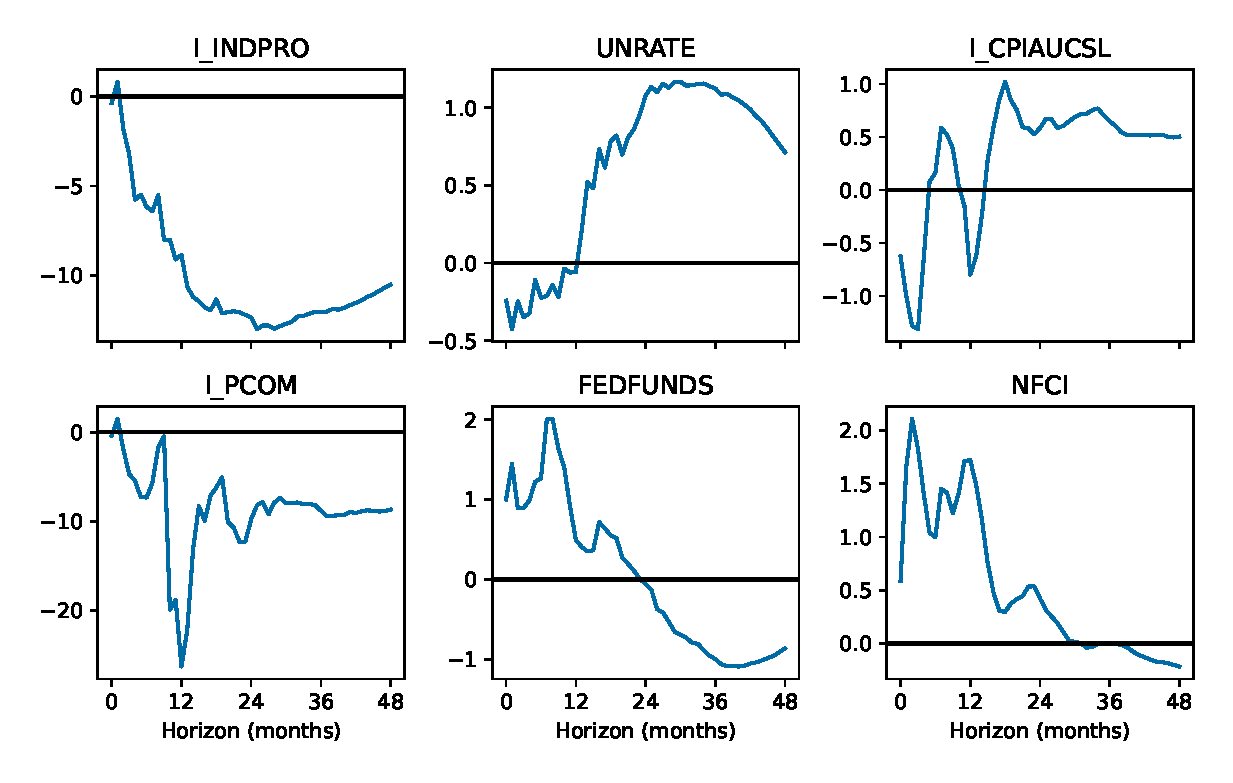
\includegraphics[width=\linewidth]{fig/mpshock_proxy_irf.eps}
\end{figure}
}

\frame{
\frametitle{Proxies (cont.)}
\begin{itemize}
\item Warning: in the literature, people also use an alternative approach to proxy identification that does not directly put $z_t$ in the estimated VAR.
\item Instead, they estimate a VAR without $z_t$ first, yielding residuals $\hat{\bm{u}}_t$. Subsequently, they regress $z_t$ on $\hat{\bm{u}}_t$ to identify the shock of interest.
\item This latter approach is sometimes called ``proxy-SVAR'' or ``SVAR with external instrument''. This approach requires more assumptions than the method that just puts $z_t$ in the VAR and orders it first, which is sometimes called ``SVAR with \textbf{internal instrument}''.
\item For details, see Stock \& Watson (2018) on the reading list.
\end{itemize}
}

\frame{
\frametitle{LP vs.\ VAR}
\begin{itemize}
\item Both LPs and VARs can be used to estimate IRFs and FEVDs, with either observed shocks, timing restrictions, or proxies.
\item \alert{Result:} in large samples, the LP-estimated IRFs approximately coincide with the VAR-estimated IRFs at horizons $h \leq p$, where $p$ is the number of lagged controls.
\item At longer horizons, the two methods can differ substantially:
\begin{itemize}
\item The SVAR estimate $\hat{\bm{\Theta}}_h = \hat{\bm{A}}^h \hat{\bm{H}}$ \textbf{extrapolates} the responses at horizons $h \geq p+1$ from the sample autocovariances at lags $1,2,\dots,p$.
\item The LP estimate directly uses the sample autocovariance $\widehat{\cov}(y_{i,t+h},\tilde{x}_t)$ out to the horizon $h$ of interest.
\end{itemize}
\end{itemize}
}

\frame{
\frametitle{LP vs.\ VAR: recursive identification}
\begin{itemize}
\item As we've seen, both LP and SVAR can be used for single-shock recursive identification (timing restrictions).
\item Given your timing assumptions, whatever variables you would order \emph{before} the policy variable in an SVAR should be the variables that enter as \emph{contemporaneous} controls in an LP.
\item Monetary policy shock application: LP regresses future outcomes on FEDFUNDS, controlling for\dots
\begin{itemize}
\item \emph{Contemporaneous} values of INDPRO, UNRATE, CPI, PCOM.
\item \emph{Lagged} values of all six time series.
\end{itemize}
\end{itemize}
}

\frame{
\begin{center}
\textbf{IRF of INDPRO to MP shock (unit effect normalization)}
\end{center}
\vspace{-0.5\baselineskip}
\begin{figure}
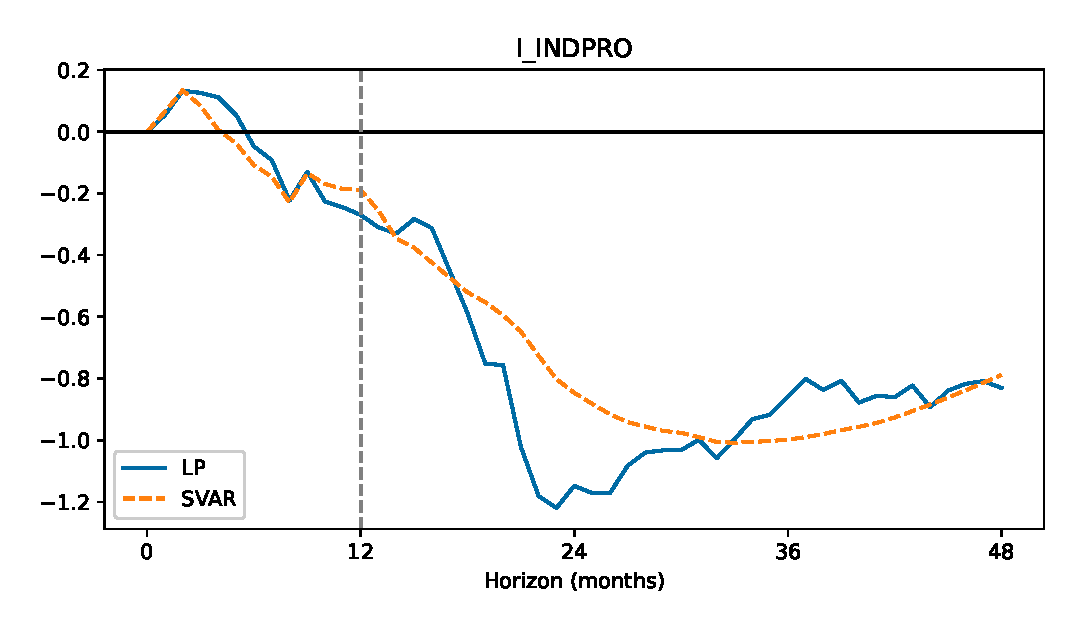
\includegraphics[width=\linewidth]{fig/mpshock_lp_svar.eps} \\
\medskip
\small
Recursive identification, normalizing impact FEDFUNDS response to 1 \\[0.2\baselineskip]
Vertical line marks lag length $p=12$
\end{figure}
}

\frame{
\frametitle{LP vs.\ VAR: bias-variance trade-off}
\begin{itemize}
\item There is no meaningful distinction between LP and VAR if we control for many lags $p$.
\item For a smaller number of lags $p$, there is a \textbf{bias-variance trade-off}:
\begin{itemize}
\item Since SVAR extrapolates, it's more exposed to bias if we get the lag length or set of controls slightly wrong.
\item For the same reason, SVAR has lower variance than LP: sample autocovariances at short lags more precisely estimated than at long lags.
\end{itemize}
\item The choice of LP vs.\ VAR therefore comes down to your taste for bias vs.\ variance.
\item However, when it comes to \emph{confidence intervals}, the choice is clear: the LP interval has more accurate coverage. This is because the biased SVAR estimate can seriously degrade the coverage.
\end{itemize}
}

\frame{
\frametitle{LP vs.\ VAR: recommendation}
\begin{itemize}
\item Macro data sets are small, so estimation uncertainty is often large.
\item We therefore want accurate uncertainty assessments, i.e., confidence intervals with accurate coverage.
\item My recommendation: use LP.
\begin{itemize}
\item This is just for estimating dynamic causal effects. VARs with small/moderate lag length are still very useful for forecasting!
\end{itemize}
\item Alternatively, you could use an SVAR with a very large lag length (many more than what AIC typically selects). Compare your results to LP -- if they are different, include more lags.
\item Further discussion: Montiel Olea et al.\ (2026) on the reading list.
\end{itemize}
}

\frame{
\frametitle{Other identification approaches}
\begin{itemize}
\item If you read papers, you will see other ways of identifying IRFs, including (but not limited to):
\end{itemize}
\medskip
\begin{enumerate}
\item \textbf{Long-run restrictions:} restrict which variables can respond to which shocks in the \emph{long run} (as opposed to on impact).
\begin{itemize}
\item Can be quite sensitive -- difficult to robustly estimate long-run responses.
\end{itemize}
\item \textbf{Sign restrictions:} rather than assuming that certain impact responses are zero, we assume that we know the \emph{signs} (positive/negative) of certain responses.
\begin{itemize}
\item Often easier to justify based on economic theory. But inference is \emph{very} tricky, and many papers get it wrong!
\end{itemize}
\end{enumerate}
\medskip
\begin{itemize}
\item If you want to delve into this, ask me!
\end{itemize}
}

\frame{
\frametitle{What did we learn?}
\begin{itemize}
\item SVAR
\begin{itemize}
\item IRF, FEVD
\item Identification problem
\item Timing assumptions (Cholesky, recursive)
\item Directly measured shock, proxy
\end{itemize}
\item LP vs.\ VAR
\begin{itemize}
\item Similar with large $p$, bias-variance trade-off with small/moderate $p$
\item Choose LP (or VAR with large $p$) for accurate conf.\ interval coverage
\end{itemize}
\item Other identification approaches
\end{itemize}
}

\frame{
\frametitle{Looking ahead}
\begin{itemize}
\item Using prior information to reduce the variance of VAR forecasts/IRFs
\item Bayesian inference with Stan
\end{itemize}
}

\end{document}
